\documentclass[11pt]{article}

\usepackage[utf8]{inputenc}
\usepackage[T1]{fontenc}
\usepackage{lmodern}
\usepackage{amsmath, amssymb}
\usepackage{xcolor}
\usepackage{tcolorbox}
\usepackage{graphicx}
\usepackage{tikz}
\usepackage{float}
\usepackage{hyperref}
\usepackage{enumitem}
\usepackage{caption}
\usepackage[margin=1in]{geometry}

\usetikzlibrary{shapes, arrows.meta, positioning}

\hypersetup{
  colorlinks=true,
  linkcolor=blue,
  urlcolor=blue,
  citecolor=blue
}


% --- Semantic tcolorbox styles ---
\definecolor{defblue}{RGB}{41, 98, 163}
\definecolor{insightgreen}{RGB}{46, 139, 87}
\definecolor{warnorange}{RGB}{204, 119, 34}
\definecolor{recapgray}{RGB}{100, 100, 100}
\definecolor{actionviolet}{RGB}{106, 61, 154}
\definecolor{resultteal}{RGB}{0, 128, 128}

\newtcolorbox{defbox}[1][]{colback=defblue!5!white, colframe=defblue!80, fonttitle=\bfseries, #1}
\newtcolorbox{insightbox}[1][]{colback=insightgreen!5!white, colframe=insightgreen!80, fonttitle=\bfseries, #1}
\newtcolorbox{warnbox}[1][]{colback=warnorange!6!white, colframe=warnorange!80, fonttitle=\bfseries, #1}
\newtcolorbox{recapbox}[1][]{colback=recapgray!6!white, colframe=recapgray!70, fonttitle=\bfseries, #1}
\newtcolorbox{actionbox}[1][]{colback=actionviolet!5!white, colframe=actionviolet!70, fonttitle=\bfseries, #1}
\newtcolorbox{resultbox}[1][]{colback=resultteal!5!white, colframe=resultteal!80, fonttitle=\bfseries, #1}


% --- TikZ diagram colors ---
\definecolor{inputblue}{RGB}{41, 98, 163}
\definecolor{neuronorange}{RGB}{230, 140, 30}
\definecolor{activgreen}{RGB}{46, 139, 87}
\definecolor{outputviolet}{RGB}{106, 61, 154}
\definecolor{arrowgray}{RGB}{80, 80, 80}
\definecolor{layer1color}{RGB}{41, 98, 163}
\definecolor{layer2color}{RGB}{204, 119, 34}
\definecolor{outputlayercolor}{RGB}{0, 128, 128}
\begin{document}

\begin{titlepage}
    \centering
    \vspace*{2.2cm}

    {\Large \textbf{DEEP LEARNING FROM SCRATCH}}\\[0.4em]
    A Guide for Self-Learners\\[2.5em]

    {\Huge \bfseries Episode V}\\[0.4em]
    {\LARGE \textit{The Rise of Intelligence}}\\[2em]

    \vspace{0.8cm}

    {\large\itshape
    You've always wanted to understand how neural networks really work.\\
    But every resource is either too shallow or a 200-page textbook.\\[0.8em]
    {\Large \textbf{This is neither.}}
    }

    \vspace{0.8cm}

    \begin{tcolorbox}[colback=black!3!white, colframe=black!20!white, width=0.8\textwidth, sharp corners, boxrule=0.4pt]
    \centering
    \itshape

    {\Large The math is tough, but you only need to do it once.}\\[1em]

    \textbf{Why this episode?}\\[0.3em]
    We go deep into the real equations.\\
    Forward propagation, backpropagation, gradients.\\
    No shortcuts. No hand-waving. Just honest computation.
    \end{tcolorbox}

    \vspace{1.5cm}

    \begin{center}
    \itshape
        {\Large \textit{``What I cannot create, I do not understand.''}}\\
        \vspace{0.2em}
        {\large -- Richard Feynman}
    \end{center}

    \vfill

    {\large \textbf{Pierre Chambet}}\\[0.3em]
    {\small March 2026}\\[1em]
    \rule{0.8\textwidth}{0.4pt}\\[0.4em]
    {\small Part of the \textit{Deep Learning From Scratch} series --- an independent reconstruction of AI.}

\end{titlepage}

\tableofcontents

\vspace{1.5em}

\begin{defbox}[title=What You'll Learn in This Episode]
After these 25 pages, you won't just know what a neural network is --- you'll know \textit{how it thinks}, \textit{how it learns}, and \textit{how to build one yourself}.

\begin{enumerate}[label=\textbf{\arabic*.}]
  \item Why a single neuron isn't enough --- and what deep learning does about it
  \item How to build a \textbf{layer} of neurons using matrix operations: $Z = Wx + b$
  \item What an \textbf{activation function} does and why it matters
  \item How to stack layers into a \textbf{deep neural network}
  \item The complete \textbf{forward propagation} pipeline
  \item The full derivation of \textbf{backpropagation} --- every gradient, step by step
  \item The final gradient equations you'll implement in code
\end{enumerate}
\end{defbox}

\newpage

\section{Theory of Neural Networks}

In the previous episode, we trained a single neuron.
It worked --- on simple data.
But it hit a wall: one neuron can only draw one straight line.
That's not enough for real problems.

\textit{Today, we break through that wall.}

\begin{recapbox}[title=What's Ahead]
This episode is about the \textbf{real math} behind neural networks.
It's dense. It's honest. And you only need to do it \textbf{once}.

After this, you'll understand what every framework hides from you ---
and that understanding is what separates someone who uses tools
from someone who can \textit{build} them.
\end{recapbox}

Remember --- a data scientist is not a mathematician.
They rarely compute things by hand. Instead, they rely on libraries to do the heavy lifting.
So, your job is simple: understand it deeply, once and for all. After that, you're good.

\textbf{And that's the beauty of it:} very few people truly understand what's going on behind the scenes.
But those who do? They're the ones capable of designing their own models and architectures.

\begin{actionbox}[title=Let's Begin]
No more talking --- let's dive into the theory of neural networks.
\end{actionbox}

We’ve already encountered the concept of a neuron through the perceptron model.

\begin{itemize}
  \item It takes multiple inputs,
  \item Applies weights,
  \item Produces an output using a threshold activation function.
\end{itemize}

This is the foundation.  
And yes, the perceptron can classify data into two categories — but it quickly reaches its limits.  
\textbf{It’s not powerful enough} for real-world complexity.

\section{Machine Learning Approach}

To overcome this, traditional \textbf{machine learning} applies a clever workaround.  
We enrich the input space with manually engineered features: things like $x_1^2$, $x_2^2$, $x_1x_2$, and so on.

This transforms a linear model into a more flexible one — usually polynomial.  
The process is called \textit{feature engineering}.

\begin{warnbox}[title=Feature Engineering]
The art of creating new features from existing ones — based on domain knowledge, intuition, and a bit of trial-and-error.
\end{warnbox}

It works — but it’s manual, tedious, and not scalable to complex data.

\section{Deep Learning Approach}

Deep learning asks a new question:

\begin{quote}
\textbf{What if... we connected neurons together?}
\end{quote}

Instead of manually building features, we let the network \textit{learn them itself}.

How?

We stack layers of neurons — one after the other — forming what we call a \textbf{deep neural network}.  
Each layer learns to extract more abstract, more meaningful representations from the previous one.

\textit{This is the essence of deep learning:}

\begin{insightbox}[title=Key Idea]
Let the model automatically learn the best features by stacking multiple layers of neurons.
\end{insightbox}

Each transformation brings us closer to understanding the data.  
Each layer does a little more, building up to a powerful representation.

In the end, the model becomes capable of learning incredibly complex functions —  
\textbf{and making remarkably accurate predictions.}

Sounds intense?

\textbf{Good.} That’s how you know it’s worth it.

\begin{quote}
We’re going to build a neural network from scratch — using math and matrix operations.
\end{quote}

\section{Let's Go}

We’re not here to waste time.  
Let’s take the neuron we previously built — and simply \textbf{duplicate it}.

We now have two neurons: $N_1$ and $N_2$, placed side by side.  
And just like that, we’ve built our first:

\begin{center}
    \textbf{\Large Layer}
\end{center}

\begin{figure}[H]
    \centering
    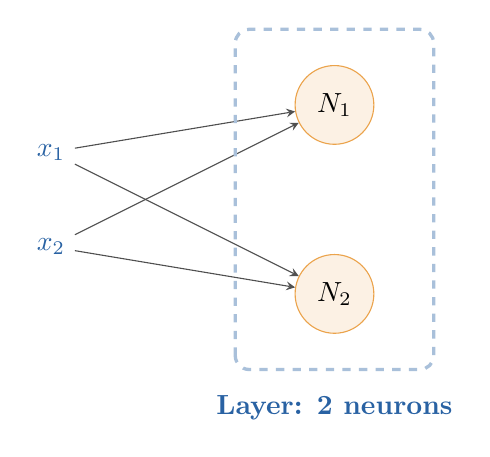
\begin{tikzpicture}[x=1.8cm, y=1.2cm, >=stealth]
    
    % Inputs
    \node[font=\bfseries, text=inputblue] at (0,2) (x1) {$x_1$};
    \node[font=\bfseries, text=inputblue] at (0,1) (x2) {$x_2$};
    
    % First neuron N1
    \node[circle,draw=neuronorange!80,fill=neuronorange!12,minimum size=1cm] at (2,2.5) (N1) {$N_1$};
    \draw[->,arrowgray] (x1) -- (N1);
    \draw[->,arrowgray] (x2) -- (N1);
    
    % Second neuron N2
    \node[circle,draw=neuronorange!80,fill=neuronorange!12,minimum size=1cm] at (2,0.5) (N2) {$N_2$};
    \draw[->,arrowgray] (x1) -- (N2);
    \draw[->,arrowgray] (x2) -- (N2);
    
    % Layer box
    \draw[dashed,rounded corners=5pt,layer1color!40,line width=1.2pt] (1.3,-0.3) rectangle (2.7,3.3);
    \node[text=layer1color] at (2,-0.7) {\textbf{Layer: 2 neurons}};
    
    \end{tikzpicture}
    \caption{A layer groups multiple neurons — each with its own weights and bias — but sharing the same input.}
\end{figure}

\subsection{What Is a Layer?}

A \textbf{layer} is simply a collection of neurons that operate \textit{in parallel}.  
They all receive the same input vector, but each computes something slightly different.

\begin{itemize}
  \item Each neuron has its own weight vector and bias.
  \item Each neuron produces one output.
\end{itemize}

So here, with $N_1$ and $N_2$, we’ll get two outputs: $z_1$ and $z_2$.

\subsection{Neuron by Neuron}

\textbf{Neuron $N_1$} takes the input $(x_1, x_2)$ and computes:
\[
z_1 = W_{11} \cdot x_1 + W_{12} \cdot x_2 + b_1
\]

Where:
\begin{itemize}
  \item $W_{11}$ and $W_{12}$ are the weights of $N_1$,
  \item $b_1$ is its bias.
\end{itemize}

\textbf{Neuron $N_2$} does the exact same thing — but with different weights and bias:
\[
z_2 = W_{21} \cdot x_1 + W_{22} \cdot x_2 + b_2
\]

So even though they process the same input, the result is different — because their parameters are different.

This is the power of layers: many neurons, one input, multiple outputs.

\subsection{The Output Equation — Matrix Form}

Now let’s write all of this in a single, elegant expression:

\[
\begin{bmatrix}
z_1 \\
z_2
\end{bmatrix}
=
\begin{bmatrix}
W_{11} & W_{12} \\
W_{21} & W_{22}
\end{bmatrix}
\begin{bmatrix}
x_1 \\
x_2
\end{bmatrix}
+
\begin{bmatrix}
b_1 \\
b_2
\end{bmatrix}
\]

Or, more compactly:
\[
Z = W x + b
\]

\begin{defbox}[title=Notation Guide]
\begin{itemize}
  \item $x$ is the input vector (shared by all neurons),
  \item $W$ is the weight matrix — each row is a neuron,
  \item $b$ is the bias vector,
  \item $Z$ is the output vector of the layer.
\end{itemize}
\end{defbox}

\begin{insightbox}[title=Key Insight]
The matrix equation $Z = Wx + b$ allows us to compute the output of the whole layer in one step —  
it’s the vectorized form of everything we just did manually.
\end{insightbox}

\section{Activation Function}

We’re almost there.  
Now that our neurons have computed their raw outputs $z_1$ and $z_2$, we apply a final transformation:

\begin{center}
    \textbf{The activation function.}
\end{center}

Why?  
Because we want to introduce \textbf{non-linearity} into our model —  
so it can learn complex patterns, not just straight lines.

\begin{defbox}[title=Sigmoid Activation Function]
The sigmoid is a classic choice:
\[
a(z) = \frac{1}{1 + e^{-z}}
\]

It maps any real number to a value between $0$ and $1$.  
Perfect when we want to interpret outputs as probabilities.
\end{defbox}

We apply the sigmoid to each neuron's output individually:

\[
A = a(Z)
\quad \Rightarrow \quad
\begin{bmatrix}
a_1 \\
a_2
\end{bmatrix}
=
\begin{bmatrix}
a(z_1) \\
a(z_2)
\end{bmatrix}
=
\begin{bmatrix}
\frac{1}{1 + e^{-z_1}} \\
\frac{1}{1 + e^{-z_2}}
\end{bmatrix}
\]

Here, $a_1$ and $a_2$ are the \textbf{activated outputs} of neurons $N_1$ and $N_2$.

\begin{insightbox}[title=Key Insight]
Each neuron computes its own linear combination: $z = Wx + b$  
Then applies an activation: $a = \sigma(z)$  
The result: nonlinear, learnable, expressive outputs.
\end{insightbox}

\subsection{Visual Summary}

Here is what we’ve just built — a layer of two neurons with activation functions:

\begin{figure}[H]
\centering
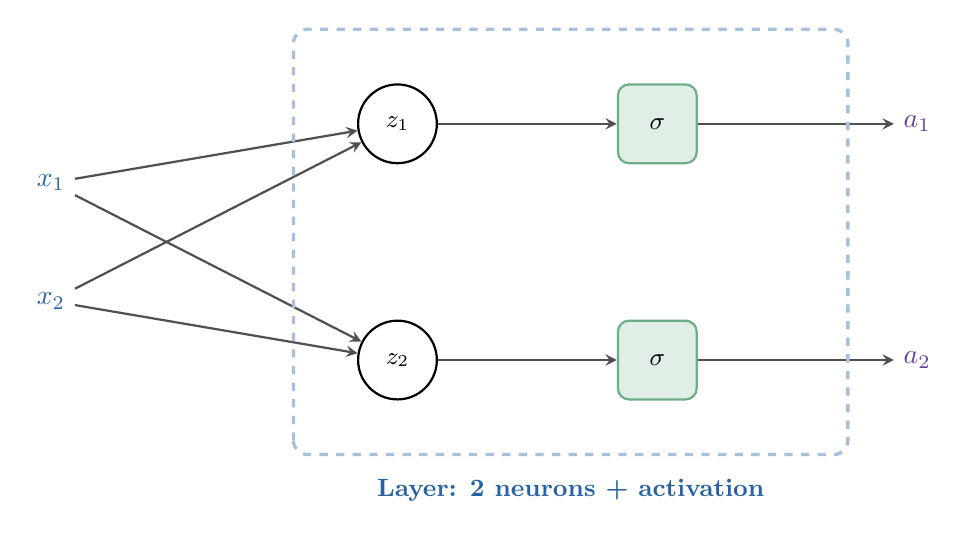
\begin{tikzpicture}[x=2.2cm, y=1.5cm, >=stealth, every node/.style={font=\small}]

% Input nodes
\node[font=\bfseries, text=inputblue] at (0,2) (x1) {$x_1$};
\node[font=\bfseries, text=inputblue] at (0,1) (x2) {$x_2$};

% Neurons z (linear)
\node[circle,draw,minimum size=1cm,thick] at (2,2.5) (N1) {$z_1$};
\node[circle,draw,minimum size=1cm,thick] at (2,0.5) (N2) {$z_2$};

% Activation function blocks
\node[rectangle,draw,minimum height=1cm,minimum width=1cm,thick,rounded corners=4pt,fill=activgreen!15,draw=activgreen!70] at (3.5,2.5) (A1) {$\sigma$};
\node[rectangle,draw,minimum height=1cm,minimum width=1cm,thick,rounded corners=4pt,fill=activgreen!15,draw=activgreen!70] at (3.5,0.5) (A2) {$\sigma$};

% Activated outputs
\node[text=outputviolet,font=\bfseries] at (5,2.5) (a1) {$a_1$};
\node[text=outputviolet,font=\bfseries] at (5,0.5) (a2) {$a_2$};

% Connections: x to z
\draw[->,thick,arrowgray] (x1) -- (N1);
\draw[->,thick,arrowgray] (x2) -- (N1);
\draw[->,thick,arrowgray] (x1) -- (N2);
\draw[->,thick,arrowgray] (x2) -- (N2);

% Connections: z to sigma
\draw[->,thick,arrowgray] (N1) -- (A1);
\draw[->,thick,arrowgray] (N2) -- (A2);

% Connections: sigma to activated output
\draw[->,thick,arrowgray] (A1) -- (a1);
\draw[->,thick,arrowgray] (A2) -- (a2);

% Layer box
\draw[dashed,rounded corners=5pt,layer1color!40,line width=1.2pt] (1.4,-0.3) rectangle (4.6,3.3);
\node[text=layer1color] at (3,-0.6) {\textbf{Layer: 2 neurons + activation}};
\end{tikzpicture}
\caption{Each neuron computes $z = Wx + b$, then applies $\sigma(z)$ to produce its final output $a$.}
\end{figure}

\subsection{Very Important}

\begin{quote}
\textbf{The outputs of the activation function are the true outputs of the layer.}  

In our case, we now have two activated outputs:  
\[
\boxed{a_1 \quad \text{and} \quad a_2}
\]
These form the output vector of the first layer.
\end{quote}

\section{Adding Neurons in the Layer}

Let’s say we want more power.  
What’s stopping us from adding more neurons to the layer?

\begin{recapbox}[title=Answer]
\textbf{Nothing.} We just add more rows to the weight matrix, and more entries in the bias vector.
\end{recapbox}

Here’s what that looks like:

\[
W =
\begin{bmatrix}
W_{11} & W_{12} \\
W_{21} & W_{22} \\
W_{31} & W_{32}
\end{bmatrix}
\quad \text{and} \quad
b =
\begin{bmatrix}
b_1 \\
b_2 \\
b_3
\end{bmatrix}
\]

Same input $x$, same formula:
\[
Z = W x + b
\]

Now, the output becomes:

\[
\begin{bmatrix}
z_1 \\
z_2 \\
z_3
\end{bmatrix}
=
\begin{bmatrix}
W_{11} & W_{12} \\
W_{21} & W_{22} \\
W_{31} & W_{32}
\end{bmatrix}
\begin{bmatrix}
x_1 \\
x_2
\end{bmatrix}
+
\begin{bmatrix}
b_1 \\
b_2 \\
b_3
\end{bmatrix}
\]

Each new row corresponds to a new neuron, with its own weights and bias.  
The logic remains exactly the same.

\begin{quote}
\textbf{We can add 3, 10, 100 neurons — as many as we want — and the equation stays the same.}
\end{quote}

\begin{figure}[H]
\centering
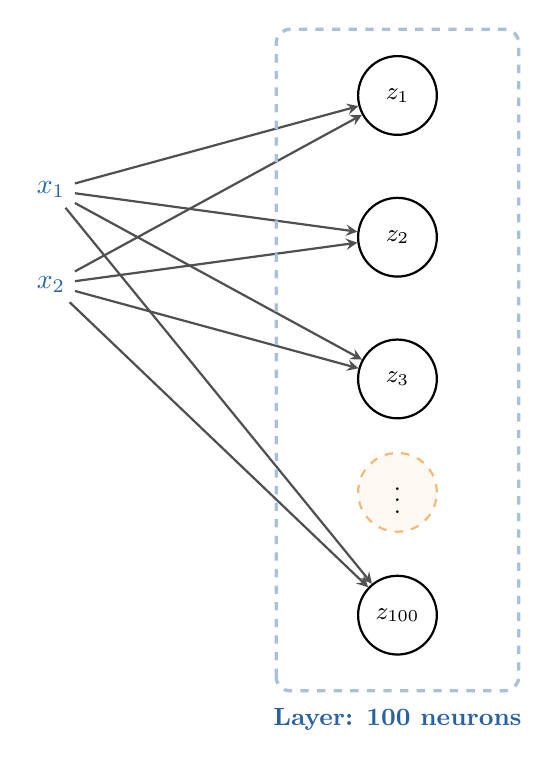
\begin{tikzpicture}[x=2.2cm, y=1.2cm, >=stealth, every node/.style={font=\small}]

% Inputs
\node[font=\bfseries, text=inputblue] at (0,3) (x1) {$x_1$};
\node[font=\bfseries, text=inputblue] at (0,2) (x2) {$x_2$};

% Neurons z (linear)
\node[circle,draw,minimum size=1cm,thick] at (2,4) (N1) {$z_1$};
\node[circle,draw,minimum size=1cm,thick] at (2,2.5) (N2) {$z_2$};
\node[circle,draw,minimum size=1cm,thick] at (2,1) (N3) {$z_3$};
\node[circle,draw=neuronorange!60,fill=neuronorange!6,minimum size=1cm,thick,dashed] at (2,-0.2) (Ndots) {$\vdots$};
\node[circle,draw,minimum size=1cm,thick] at (2,-1.5) (N6) {$z_{100}$};

% Connections (show to 3 neurons only)
\foreach \target in {N1,N2,N3,N6} {
    \draw[->,thick,arrowgray] (x1) -- (\target);
    \draw[->,thick,arrowgray] (x2) -- (\target);
}

% Layer box
\draw[dashed,rounded corners=5pt,layer1color!40,line width=1.2pt] (1.3,-2.3) rectangle (2.7,4.7);
\node[text=layer1color] at (2,-2.6) {\textbf{Layer: 100 neurons}};
\end{tikzpicture}
\caption{A layer with 100 neurons — each receiving the same input, but with its own weights and bias.}
\end{figure}
\section{A Layer is a Collection of Neurons}

Let’s take a step back and reframe what a layer really is.

A \textbf{layer} is just a collection of neurons working in parallel.  
It takes an input, and produces multiple outputs — one from each neuron.  

\begin{insightbox}[title=Analogy]
You can think of a layer as one giant neuron —  
but made of many smaller neurons, each with its own weights and bias.
\end{insightbox}

For now, we’re working with two neurons in our first layer.

We now introduce the notation for layers explicitly.  
The output of the first layer — after applying the activation — is written as:

\[
A = A_1 = 
\begin{bmatrix}
a_1 \\
a_2
\end{bmatrix}
= a(Z_1) =
\begin{bmatrix}
a(z_1) \\
a(z_2)
\end{bmatrix}
\]

Where:
\begin{itemize}
  \item $Z_1$ is the pre-activation output of the first layer (before sigmoid),
  \item $A_1$ is the activated output of the first layer,
  \item $a_1$ and $a_2$ are the outputs of neurons $N_1$ and $N_2$ after activation.
\end{itemize}

\section{Adding a Second Layer}

Now, something exciting happens.

We’re no longer going to feed the raw input $x$ to the layer —  
we’re going to feed it the output of the previous layer: $A_1$.

\begin{defbox}[title=Deep Architecture]
\begin{itemize}
    \item The first layer takes the original input $x$ and produces $A_1$.
    \item The second layer takes $A_1$ as input and produces $A_2$.
\end{itemize}
\end{defbox}

Let’s keep it simple for now.  
\textbf{We’ll add just one neuron in the second layer.}

This neuron will:
\begin{itemize}
  \item Take $a_1$ and $a_2$ as inputs,
  \item Apply its own weights and bias,
  \item Produce a pre-activation $z_3$,
  \item Then apply the activation to get $a_3$.
\end{itemize}

\[
z_3 = W_{31} \cdot a_1 + W_{32} \cdot a_2 + b_3
\quad \Rightarrow \quad
a_3 = \sigma(z_3)
\]

So now we have:

\[
A_2 =
\begin{bmatrix}
a_3
\end{bmatrix}
\]

\begin{warnbox}[title=Important Insight]
Each new layer takes the output of the previous layer as input.  
This stacking is what gives neural networks their depth — and power.
\end{warnbox}
\begin{figure}[H]
\centering
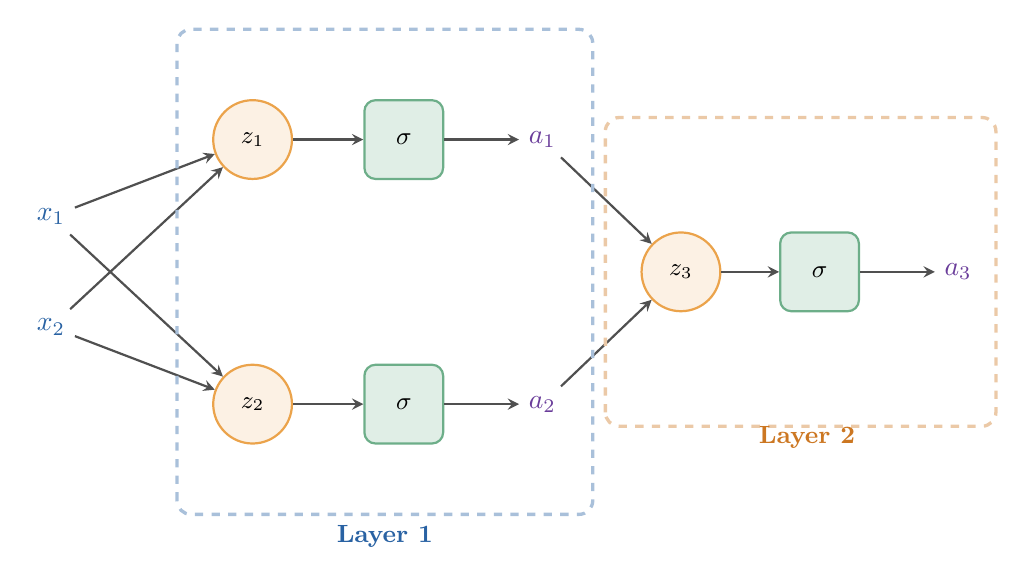
\begin{tikzpicture}[x=1.6cm, y=1.4cm, >=stealth, every node/.style={font=\small}]

% Inputs
\node[font=\bfseries, text=inputblue] at (0,3) (x1) {$x_1$};
\node[font=\bfseries, text=inputblue] at (0,2) (x2) {$x_2$};

% Hidden layer z
\node[circle,draw=neuronorange!80,fill=neuronorange!12,thick,minimum size=1cm] at (1.6,3.7) (z1) {$z_1$};
\node[circle,draw=neuronorange!80,fill=neuronorange!12,thick,minimum size=1cm] at (1.6,1.3) (z2) {$z_2$};

% Activations a1 and a2
\node[rectangle,draw,rounded corners=4pt,thick,fill=activgreen!15,draw=activgreen!70,minimum size=1cm] at (2.8,3.7) (a1) {$\sigma$};
\node[rectangle,draw,rounded corners=4pt,thick,fill=activgreen!15,draw=activgreen!70,minimum size=1cm] at (2.8,1.3) (a2) {$\sigma$};

% Activated outputs
\node[text=outputviolet,font=\bfseries] at (3.9,3.7) (a1_out) {$a_1$};
\node[text=outputviolet,font=\bfseries] at (3.9,1.3) (a2_out) {$a_2$};

% Second layer z3
\node[circle,draw=neuronorange!80,fill=neuronorange!12,thick,minimum size=1cm] at (5,2.5) (z3) {$z_3$};

% Activation a3
\node[rectangle,draw,rounded corners=4pt,thick,fill=activgreen!15,draw=activgreen!70,minimum size=1cm] at (6.1,2.5) (a3) {$\sigma$};

% Output a3
\node[text=outputviolet,font=\bfseries] at (7.2,2.5) (a3_out) {$a_3$};

% Connections: input to layer 1
\foreach \target in {z1,z2} {
  \draw[->,thick,arrowgray] (x1) -- (\target);
  \draw[->,thick,arrowgray] (x2) -- (\target);
}

% Connections: z to activation
\draw[->,thick,arrowgray] (z1) -- (a1);
\draw[->,thick,arrowgray] (z2) -- (a2);

% Connections: activation to a1_out
\draw[->,thick,arrowgray] (a1) -- (a1_out);
\draw[->,thick,arrowgray] (a2) -- (a2_out);

% Connections: a1 and a2 to z3
\draw[->,thick,arrowgray] (a1_out) -- (z3);
\draw[->,thick,arrowgray] (a2_out) -- (z3);

% z3 to a3 to final output
\draw[->,thick,arrowgray] (z3) -- (a3);
\draw[->,thick,arrowgray] (a3) -- (a3_out);

% Layer boxes
\draw[dashed,layer1color!40,rounded corners=5pt,line width=1.2pt] (1,0.3) rectangle (4.3,4.7);
\node[text=layer1color] at (2.65,0.1) {\textbf{Layer 1}};

\draw[dashed,layer2color!40,rounded corners=5pt,line width=1.2pt] (4.4,1.1) rectangle (7.5,3.9);
\node[text=layer2color] at (6,1) {\textbf{Layer 2}};

\end{tikzpicture}
\caption{A two-layer neural network: the output of Layer 1 becomes the input to Layer 2.}
\end{figure}

\section{Second Layer Computation}

We now know that the output of the first layer is:
\[
A_1 =
\begin{bmatrix}
a_1 \\
a_2
\end{bmatrix}
\]

Let’s feed this into the second layer.  
This time, we’ll work with a single neuron in the second layer.

\begin{defbox}[title=Layer 2 Computation]
The second layer computes:
\[
Z_2 = W_2 A_1 + b_2
\]
Where:
\begin{itemize}
  \item $W_2$ is the weight matrix of the second layer,
  \item $A_1$ is the input (from the first layer),
  \item $b_2$ is the bias of the second layer.
\end{itemize}
\end{defbox}

Then we apply the activation function:
\[
A_2 = a(Z_2)
\]

Let’s look at a concrete example.  
Suppose we have:

\[
W_2 = \begin{bmatrix} w_{21} & w_{22} \end{bmatrix}, \quad
b_2 = \begin{bmatrix} b_3 \end{bmatrix}
\]

Then:
\[
Z_2 = 
\begin{bmatrix}
z_3
\end{bmatrix}
= W_2 A_1 + b_2 = 
\begin{bmatrix}
w_{21} & w_{22}
\end{bmatrix}
\begin{bmatrix}
a_1 \\
a_2
\end{bmatrix}
+
\begin{bmatrix}
b_3
\end{bmatrix}
\]

And the final activated output becomes:

\[
A_2 = 
\begin{bmatrix}
a_3
\end{bmatrix}
= a(Z_2) = 
\begin{bmatrix}
a(z_3)
\end{bmatrix}
= \begin{bmatrix}
\frac{1}{1 + e^{-z_3}}
\end{bmatrix}
\]

This shows a full forward pass through a 2-layer neural network.  
From $x \rightarrow A_1 \rightarrow A_2$, the data flows forward — layer by layer —  
with weights, biases, and activations applied at each stage.

\begin{insightbox}[title=Key Insight]
Each layer is a clean block: linear operation ($Wx + b$) followed by a non-linearity ($a(z)$).  
Stacking these blocks is what builds a deep neural network.
\end{insightbox}
\section{Adding More Neurons to the Second Layer}

Why stop at one neuron?

We can easily add more neurons to the second layer by:

\begin{itemize}
  \item adding more \textbf{rows} to the weight matrix $W_2$,
  \item and more \textbf{entries} to the bias vector $b_2$.
\end{itemize}

\begin{recapbox}[title={Same Logic, More Neurons}]
The matrix equation stays the same:
\[
Z_2 = W_2 A_1 + b_2
\]
\end{recapbox}

Let’s say we now have \textbf{three neurons} in the second layer.  
The output becomes:

\[
A_2 = 
\begin{bmatrix}
a_1 \\
a_2 \\
a_3
\end{bmatrix}
= a(Z_2) = 
a\left(
\begin{bmatrix}
z_1 \\
z_2 \\
z_3
\end{bmatrix}
\right)
=
\begin{bmatrix}
a(z_1) \\
a(z_2) \\
a(z_3)
\end{bmatrix}
\]

Each $z_i$ is computed using its own weights and bias:

\[
\begin{bmatrix}
z_1 \\
z_2 \\
z_3
\end{bmatrix}
=
\begin{bmatrix}
W_{11} & W_{12} \\
W_{21} & W_{22} \\
W_{31} & W_{32}
\end{bmatrix}
\begin{bmatrix}
a_1 \\
a_2
\end{bmatrix}
+
\begin{bmatrix}
b_1 \\
b_2 \\
b_3
\end{bmatrix}
\]

\begin{recapbox}[title=Reminder]
Each row of $W_2$ corresponds to one neuron in the layer.  
Each neuron gets the full input $A_1$ but transforms it differently.
\end{recapbox}

\subsection{Visual Recap}

Here’s what we’ve just built — a second layer with three neurons:

\begin{figure}[H]
\centering
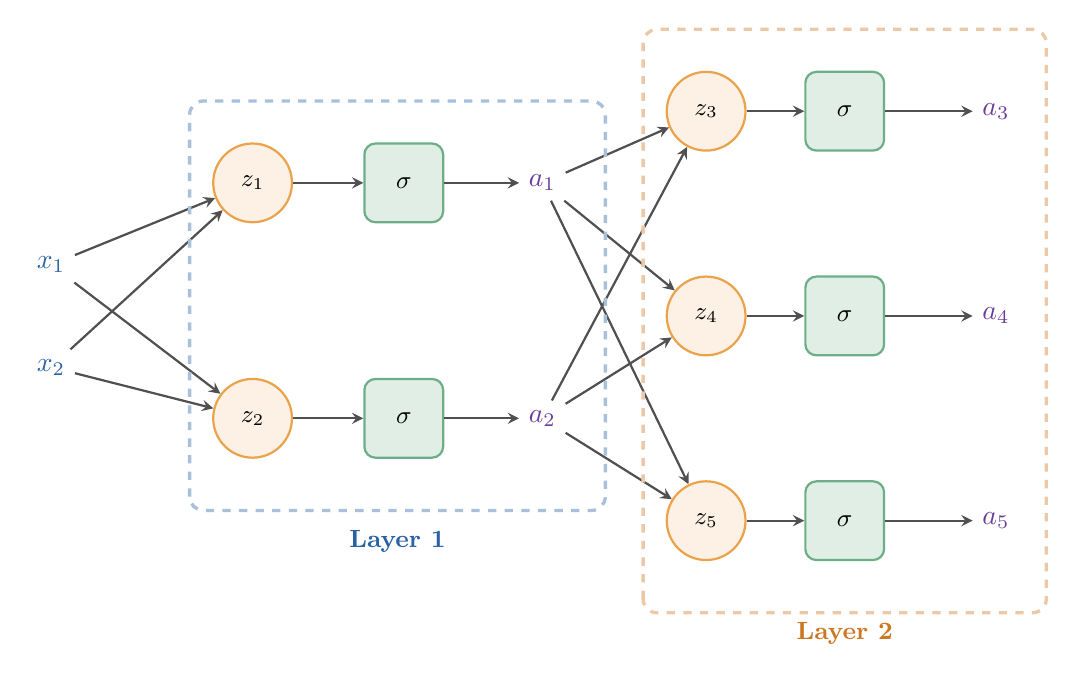
\begin{tikzpicture}[x=1.6cm, y=1.3cm, >=stealth, every node/.style={font=\small}]

% Inputs
\node[font=\bfseries, text=inputblue] at (0,3) (x1) {$x_1$};
\node[font=\bfseries, text=inputblue] at (0,2) (x2) {$x_2$};

% Layer 1 z
\node[circle,draw=neuronorange!80,fill=neuronorange!12,thick,minimum size=1cm] at (1.6,3.8) (z1) {$z_1$};
\node[circle,draw=neuronorange!80,fill=neuronorange!12,thick,minimum size=1cm] at (1.6,1.5) (z2) {$z_2$};

% Activations a1
\node[rectangle,draw,rounded corners=4pt,thick,fill=activgreen!15,draw=activgreen!70,minimum size=1cm] at (2.8,3.8) (a1) {$\sigma$};
\node[rectangle,draw,rounded corners=4pt,thick,fill=activgreen!15,draw=activgreen!70,minimum size=1cm] at (2.8,1.5) (a2) {$\sigma$};

% Layer 1 outputs
\node[text=outputviolet,font=\bfseries] at (3.9,3.8) (a1_out) {$a_1$};
\node[text=outputviolet,font=\bfseries] at (3.9,1.5) (a2_out) {$a_2$};

% Layer 2 z neurons
\node[circle,draw=neuronorange!80,fill=neuronorange!12,thick,minimum size=1cm] at (5.2,4.5) (z3) {$z_3$};
\node[circle,draw=neuronorange!80,fill=neuronorange!12,thick,minimum size=1cm] at (5.2,2.5) (z4) {$z_4$};
\node[circle,draw=neuronorange!80,fill=neuronorange!12,thick,minimum size=1cm] at (5.2,0.5) (z5) {$z_5$};

% Activations a3
\node[rectangle,draw,rounded corners=4pt,thick,fill=activgreen!15,draw=activgreen!70,minimum size=1cm] at (6.3,4.5) (a3) {$\sigma$};
\node[rectangle,draw,rounded corners=4pt,thick,fill=activgreen!15,draw=activgreen!70,minimum size=1cm] at (6.3,2.5) (a4) {$\sigma$};
\node[rectangle,draw,rounded corners=4pt,thick,fill=activgreen!15,draw=activgreen!70,minimum size=1cm] at (6.3,0.5) (a5) {$\sigma$};

% Outputs a3, a4, a5
\node[text=outputviolet,font=\bfseries] at (7.5,4.5) (a3_out) {$a_3$};
\node[text=outputviolet,font=\bfseries] at (7.5,2.5) (a4_out) {$a_4$};
\node[text=outputviolet,font=\bfseries] at (7.5,0.5) (a5_out) {$a_5$};

% Connections: x to z1, z2
\foreach \target in {z1,z2} {
  \draw[->,thick,arrowgray] (x1) -- (\target);
  \draw[->,thick,arrowgray] (x2) -- (\target);
}

% Connections: z to activation
\draw[->,thick,arrowgray] (z1) -- (a1);
\draw[->,thick,arrowgray] (z2) -- (a2);

% Activation to output
\draw[->,thick,arrowgray] (a1) -- (a1_out);
\draw[->,thick,arrowgray] (a2) -- (a2_out);

% Layer 1 to Layer 2 z-neurons
\foreach \dest in {z3,z4,z5} {
  \draw[->,thick,arrowgray] (a1_out) -- (\dest);
  \draw[->,thick,arrowgray] (a2_out) -- (\dest);
}

% z to sigma
\draw[->,thick,arrowgray] (z3) -- (a3);
\draw[->,thick,arrowgray] (z4) -- (a4);
\draw[->,thick,arrowgray] (z5) -- (a5);

% sigma to output
\draw[->,thick,arrowgray] (a3) -- (a3_out);
\draw[->,thick,arrowgray] (a4) -- (a4_out);
\draw[->,thick,arrowgray] (a5) -- (a5_out);

% Layer boxes
\draw[dashed,layer1color!40,rounded corners=5pt,line width=1.2pt] (1.1,0.6) rectangle (4.4,4.6);
\node[text=layer1color] at (2.75,0.3) {\textbf{Layer 1}};

\draw[dashed,layer2color!40,rounded corners=5pt,line width=1.2pt] (4.7,-0.4) rectangle (7.9,5.3);
\node[text=layer2color] at (6.3,-0.6) {\textbf{Layer 2}};

\end{tikzpicture}
\caption{Two-layer neural network: 2 neurons in Layer 1, 3 neurons in Layer 2.}
\end{figure}

\section{Adding a Layer}

\textbf{Key distinction:}

\begin{itemize}
    \item To \textbf{add a neuron within a layer}, you simply add a new \textbf{row} to the weight matrix and a new \textbf{entry} to the bias vector.
    \item To \textbf{add a new layer}, you introduce an entirely new \textbf{weight matrix} and a new \textbf{bias vector}.
\end{itemize}

\section{Output Layer and Final Output}

The \textbf{output layer} is the last layer of the neural network.  
It takes as input the output of the last hidden layer — and produces the final prediction.

Let’s say we use the following weight matrix and bias vector:

\[
W_3 = 
\begin{bmatrix}
w_{11} & w_{12} & w_{13}
\end{bmatrix}
\quad \text{and} \quad
b_3 = 
\begin{bmatrix}
b_1
\end{bmatrix}
\]

We compute the pre-activation of the output neuron:

\[
Z_3 = 
\begin{bmatrix}
z_1
\end{bmatrix}
= W_3 A_2 + b_3 = 
\begin{bmatrix}
w_{11} & w_{12} & w_{13}
\end{bmatrix}
\begin{bmatrix}
a_1 \\
a_2 \\
a_3
\end{bmatrix}
+
\begin{bmatrix}
b_1
\end{bmatrix}
\]

Then we apply the activation function (here: sigmoid) to get the final prediction:

\[
A_3 = a(Z_3) =
\begin{bmatrix}
\frac{1}{1 + e^{-z_1}}
\end{bmatrix}
\]

\begin{figure}[H]
\centering
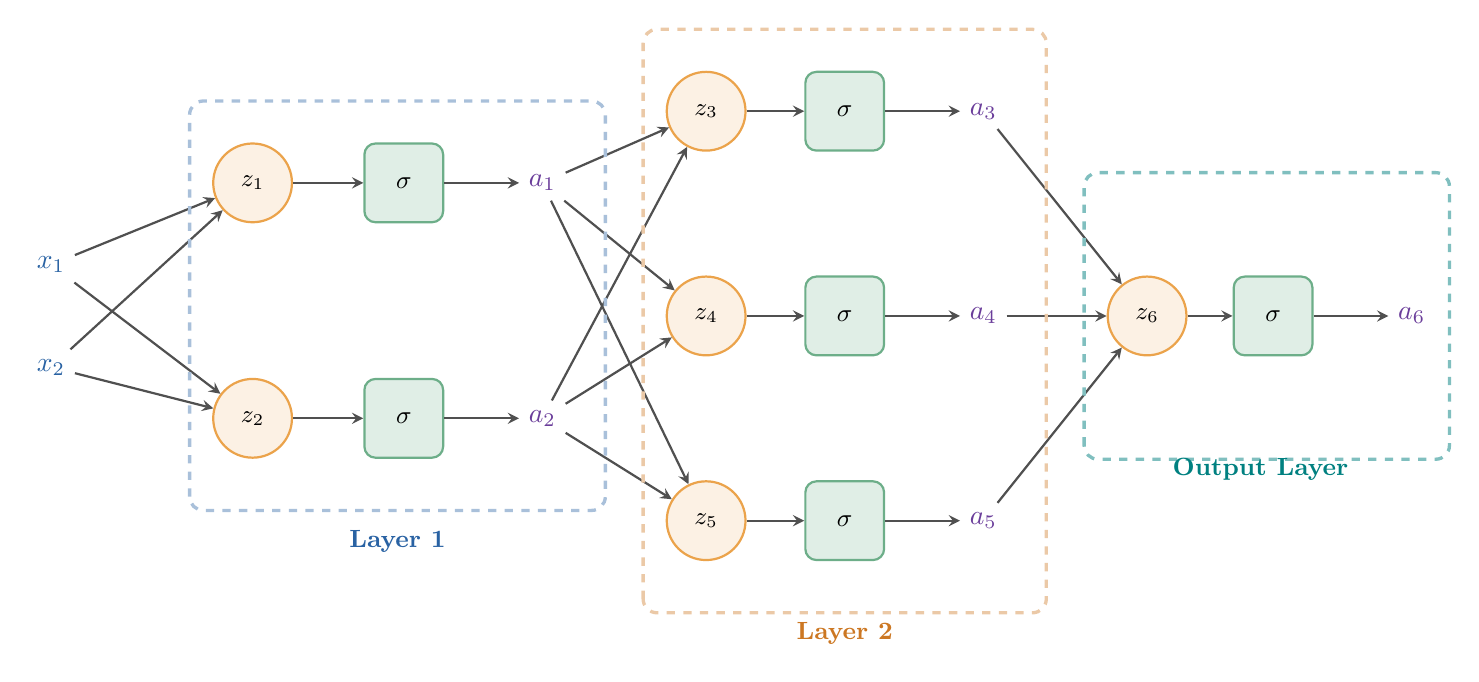
\begin{tikzpicture}[x=1.6cm, y=1.3cm, >=stealth, every node/.style={font=\small}]

% Inputs
\node[font=\bfseries, text=inputblue] at (0,3) (x1) {$x_1$};
\node[font=\bfseries, text=inputblue] at (0,2) (x2) {$x_2$};

% Layer 1 z
\node[circle,draw=neuronorange!80,fill=neuronorange!12,thick,minimum size=1cm] at (1.6,3.8) (z1) {$z_1$};
\node[circle,draw=neuronorange!80,fill=neuronorange!12,thick,minimum size=1cm] at (1.6,1.5) (z2) {$z_2$};

% Activations a1
\node[rectangle,draw,rounded corners=4pt,thick,fill=activgreen!15,draw=activgreen!70,minimum size=1cm] at (2.8,3.8) (a1) {$\sigma$};
\node[rectangle,draw,rounded corners=4pt,thick,fill=activgreen!15,draw=activgreen!70,minimum size=1cm] at (2.8,1.5) (a2) {$\sigma$};

% Outputs of layer 1
\node[text=outputviolet,font=\bfseries] at (3.9,3.8) (a1_out) {$a_1$};
\node[text=outputviolet,font=\bfseries] at (3.9,1.5) (a2_out) {$a_2$};

% Layer 2 z neurons
\node[circle,draw=neuronorange!80,fill=neuronorange!12,thick,minimum size=1cm] at (5.2,4.5) (z3) {$z_3$};
\node[circle,draw=neuronorange!80,fill=neuronorange!12,thick,minimum size=1cm] at (5.2,2.5) (z4) {$z_4$};
\node[circle,draw=neuronorange!80,fill=neuronorange!12,thick,minimum size=1cm] at (5.2,0.5) (z5) {$z_5$};

% Activations a3
\node[rectangle,draw,rounded corners=4pt,thick,fill=activgreen!15,draw=activgreen!70,minimum size=1cm] at (6.3,4.5) (a3) {$\sigma$};
\node[rectangle,draw,rounded corners=4pt,thick,fill=activgreen!15,draw=activgreen!70,minimum size=1cm] at (6.3,2.5) (a4) {$\sigma$};
\node[rectangle,draw,rounded corners=4pt,thick,fill=activgreen!15,draw=activgreen!70,minimum size=1cm] at (6.3,0.5) (a5) {$\sigma$};

% Outputs of layer 2
\node[text=outputviolet,font=\bfseries] at (7.4,4.5) (a3_out) {$a_3$};
\node[text=outputviolet,font=\bfseries] at (7.4,2.5) (a4_out) {$a_4$};
\node[text=outputviolet,font=\bfseries] at (7.4,0.5) (a5_out) {$a_5$};

% Output layer z neuron
\node[circle,draw=neuronorange!80,fill=neuronorange!12,thick,minimum size=1cm] at (8.7,2.5) (z6) {$z_6$};

% Activation
\node[rectangle,draw,rounded corners=4pt,thick,fill=activgreen!15,draw=activgreen!70,minimum size=1cm] at (9.7,2.5) (a6) {$\sigma$};

% Final output
\node[text=outputviolet,font=\bfseries] at (10.8,2.5) (a6_out) {$a_6$};

% Connections
\foreach \target in {z1,z2} {
  \draw[->,thick,arrowgray] (x1) -- (\target);
  \draw[->,thick,arrowgray] (x2) -- (\target);
}
\draw[->,thick,arrowgray] (z1) -- (a1);
\draw[->,thick,arrowgray] (z2) -- (a2);
\draw[->,thick,arrowgray] (a1) -- (a1_out);
\draw[->,thick,arrowgray] (a2) -- (a2_out);
\foreach \target in {z3,z4,z5} {
  \draw[->,thick,arrowgray] (a1_out) -- (\target);
  \draw[->,thick,arrowgray] (a2_out) -- (\target);
}
\draw[->,thick,arrowgray] (z3) -- (a3);
\draw[->,thick,arrowgray] (z4) -- (a4);
\draw[->,thick,arrowgray] (z5) -- (a5);
\draw[->,thick,arrowgray] (a3) -- (a3_out);
\draw[->,thick,arrowgray] (a4) -- (a4_out);
\draw[->,thick,arrowgray] (a5) -- (a5_out);

\foreach \src in {a3_out,a4_out,a5_out} {
  \draw[->,thick,arrowgray] (\src) -- (z6);
}
\draw[->,thick,arrowgray] (z6) -- (a6);
\draw[->,thick,arrowgray] (a6) -- (a6_out);

% Layer boxes
\draw[dashed,layer1color!40,rounded corners=5pt,line width=1.2pt] (1.1,0.6) rectangle (4.4,4.6);
\node[text=layer1color] at (2.75,0.3) {\textbf{Layer 1}};

\draw[dashed,layer2color!40,rounded corners=5pt,line width=1.2pt] (4.7,-0.4) rectangle (7.9,5.3);
\node[text=layer2color] at (6.3,-0.6) {\textbf{Layer 2}};

\draw[dashed,outputlayercolor!50,rounded corners=5pt,line width=1.2pt] (8.2,1.1) rectangle (11.1,3.9);
\node[text=outputlayercolor] at (9.6,1) {\textbf{Output Layer}};

\end{tikzpicture}
\caption{Complete neural network: 2 inputs, 2 hidden layers, 1 output neuron.}
\end{figure}

\section{Summary}

\vspace{-0.5em}

\begin{itemize}
    \item \textbf{Adding a neuron} = add a row to $W$, and an element to $b$.
    \item \textbf{Adding a layer} = create a new $W_i$ and $b_i$.
\end{itemize}

Each layer performs the same core sequence:

\begin{defbox}[title=Layer Computation --- General Rule]
\[
\text{Input:} \quad A_{i-1}
\]
\[
\text{Linear combination:} \quad Z_i = W_i A_{i-1} + b_i
\]
\[
\text{Activation:} \quad A_i = a(Z_i)
\]
\end{defbox}

\textbf{Why matrices?}  
Because they allow us to compute all neurons’ operations at once —  
fast, in parallel, and efficiently on modern hardware.

\section{Forward Propagation}

Forward propagation is the process of passing the input through the entire network —  
from the input layer, through all hidden layers, to the final output.

At each step, the same logic applies:

\begin{itemize}
    \item Apply a \textbf{linear operation} ($Z = W A + b$)
    \item Apply an \textbf{activation function} ($A = \sigma(Z)$)
\end{itemize}

This continues until we reach the final output:

\[
A_3 = \text{network prediction}
\]

\newpage

\begin{resultbox}[title=Checkpoint --- What We've Built So Far]
\textbf{Take a breath.} You've just built a complete neural network from the ground up.

Here's what you now understand:
\begin{itemize}
  \item A \textbf{layer} is a collection of neurons operating in parallel: $Z = Wx + b$
  \item An \textbf{activation function} introduces non-linearity: $A = \sigma(Z)$
  \item Stacking layers creates a \textbf{deep network}: $x \to A_1 \to A_2 \to A_3$
  \item \textbf{Forward propagation} pushes data through the entire network to produce a prediction
\end{itemize}

\textbf{Next:} we go backward --- to understand how the network \textit{learns}.
\end{resultbox}

\section{Training via Backpropagation}

Once we compute the output, we want to train the network —  
that is, adjust the weights and biases to reduce the prediction error.

To train the network, we follow these steps:

\begin{enumerate}
    \item Define a \textbf{loss function} (such as log-loss)
    \item Compute the \textbf{gradient of the loss} with respect to each parameter
    \item Update the weights and biases using \textbf{gradient descent}
\end{enumerate}

From our earlier notebook (for a single neuron), we saw:

\[
\frac{\partial \mathcal{L}}{\partial w_1} = -\frac{x_1}{m} \sum_i (y_i - a_i)
\quad\quad
\frac{\partial \mathcal{L}}{\partial w_2} = -\frac{x_2}{m} \sum_i (y_i - a_i)
\quad\quad
\frac{\partial \mathcal{L}}{\partial b} = -\frac{1}{m} \sum_i (y_i - a_i)
\]

Remember, we derived these expressions using the chain rule.

\begin{actionbox}[title=Now We Scale Up]
We will do the exact same thing here — but with \textbf{matrices}.
\end{actionbox}

\subsection{Goal: Compute the Gradients}

Let’s focus on the following parameters:

\begin{itemize}
  \item $W_1$, $b_1$ — parameters of the first layer
  \item $W_2$, $b_2$ — parameters of the second layer
\end{itemize}

Our goal is to understand how much each parameter influences the loss function.  
In other words, we want to compute:

\[
\frac{\partial \mathcal{L}}{\partial W_1}, \quad
\frac{\partial \mathcal{L}}{\partial b_1}, \quad
\frac{\partial \mathcal{L}}{\partial W_2}, \quad
\frac{\partial \mathcal{L}}{\partial b_2}
\]

As before — like we did in the perceptron model — we will use the \textbf{chain rule}.  
This time, however, we will apply it step by step through the layers of a deep network.

\begin{warnbox}[title=Before We Start]
\textbf{Read carefully. This is the foundation of the entire backward pass.}

You don’t need to memorize equations — but you must understand the logic.  
It’s all about how the functions are connected, and how parameters influence outputs.

If you get that, you’ll understand every neural network.
\end{warnbox}

\subsection{Summary of the Network Functions}

\textbf{First Layer:}
\begin{itemize}
    \item Linear transformation:
    \[
    Z_1 = W_1 X + b_1
    \]
    \item Activation:
    \[
    A_1 = \frac{1}{1 + e^{-Z_1}}
    \]
\end{itemize}

\textbf{Second Layer (Last Hidden Layer):}
\begin{itemize}
    \item Linear transformation:
    \[
    Z_2 = W_2 A_1 + b_2
    \]
    \textit{Important:} Here, the input is $A_1$, not the original input $X$.

    \item Activation:
    \[
    A_2 = \frac{1}{1 + e^{-Z_2}}
    \]

    \item Loss function:
    \[
    \mathcal{L} = -\frac{1}{m} \sum \left( y \log A_2 + (1 - y) \log(1 - A_2) \right)
    \]
    \textit{We compute the loss using $A_2$, the output of the last layer — not $A_1$.}
\end{itemize}

\section{Important}

Finding the gradients means identifying how the loss $\mathcal{L}$ depends on each parameter of the network.

But as you’ve already seen, the \textbf{entry point} between the loss $\mathcal{L}$ and the rest of the network is the output of the last layer — namely, $A_2$.

So even if we want to compute the gradients of the parameters in the \textit{first layer},  
we must first pass through the \textit{second layer}.

\begin{insightbox}[title=Key Insight]
This is the core principle of backpropagation:

\textbf{We must go backward through the network — layer by layer — to compute the gradients.}
\end{insightbox}

And when you think about it, it actually makes perfect sense.  
This is the whole point of deep learning: the model builds up its complexity layer after layer.  
So naturally, we need to go back down that stack to understand how each parameter affects the final outcome.

\section{Gradients for the Layer Just Before the Output}

Let’s now compute the gradients for the second layer, using the chain rule.

\[
\begin{aligned}
\frac{\partial \mathcal{L}}{\partial W_2} &= 
\frac{\partial \mathcal{L}}{\partial A_2} \cdot 
\frac{\partial A_2}{\partial Z_2} \cdot 
\frac{\partial Z_2}{\partial W_2} \\[1em]
\frac{\partial \mathcal{L}}{\partial b_2} &= 
\frac{\partial \mathcal{L}}{\partial A_2} \cdot 
\frac{\partial A_2}{\partial Z_2} \cdot 
\frac{\partial Z_2}{\partial b_2}
\end{aligned}
\]

Let’s break this down:

\begin{itemize}
    \item $\frac{\partial \mathcal{L}}{\partial A_2}$ is the gradient of the loss with respect to the network output
    \item $\frac{\partial A_2}{\partial Z_2}$ is the derivative of the activation function (sigmoid)
    \item $\frac{\partial Z_2}{\partial W_2}$ and $\frac{\partial Z_2}{\partial b_2}$ are the local gradients of the model
\end{itemize}

Since the first two terms appear identically in both equations, we define:

\[
dZ_2 = \frac{\partial \mathcal{L}}{\partial A_2} \cdot \frac{\partial A_2}{\partial Z_2}
\]

Then the gradients simplify to:

\[
\begin{aligned}
\frac{\partial \mathcal{L}}{\partial W_2} &= dZ_2 \cdot \frac{\partial Z_2}{\partial W_2} \\
\frac{\partial \mathcal{L}}{\partial b_2} &= dZ_2 \cdot \frac{\partial Z_2}{\partial b_2}
\end{aligned}
\]

\section{For the First Layer}

Let’s now focus on computing the gradients with respect to the parameters of the \textbf{first layer}.

Using the chain rule:

\[
\begin{aligned}
\frac{\partial \mathcal{L}}{\partial W_1} &= 
\frac{\partial \mathcal{L}}{\partial A_1} \cdot 
\frac{\partial A_1}{\partial Z_1} \cdot 
\frac{\partial Z_1}{\partial W_1} \\[1em]
\frac{\partial \mathcal{L}}{\partial b_1} &= 
\frac{\partial \mathcal{L}}{\partial A_1} \cdot 
\frac{\partial A_1}{\partial Z_1} \cdot 
\frac{\partial Z_1}{\partial b_1}
\end{aligned}
\]

Where:
\begin{itemize}
    \item $\frac{\partial \mathcal{L}}{\partial A_1}$ is the gradient of the loss with respect to the output of the first layer
    \item $\frac{\partial A_1}{\partial Z_1}$ is the derivative of the activation function
    \item $\frac{\partial Z_1}{\partial W_1}$ and $\frac{\partial Z_1}{\partial b_1}$ are the local gradients of the linear model
\end{itemize}

But — as we said before — there's a crucial observation here:

\textit{There is no direct link between the loss $\mathcal{L}$ and the output $A_1$ of the first layer.}  
To compute this gradient, we must go through the second layer — just like the signal does in the forward pass.

\begin{warnbox}[title=Pause and Think]
\textbf{How do we relate the second layer to the first?}  
What is the variable that connects both layers?

Take a moment and try to identify the link yourself.
\end{warnbox}

The answer?

It’s in the equation:

\[
Z_2 = W_2 A_1 + b_2
\]

This shows that $A_1$ is the input to the second layer.  
So to compute $\frac{\partial \mathcal{L}}{\partial A_1}$, we apply the chain rule again:

\[
\frac{\partial \mathcal{L}}{\partial A_1} = 
\frac{\partial \mathcal{L}}{\partial A_2} \cdot 
\frac{\partial A_2}{\partial Z_2} \cdot 
\frac{\partial Z_2}{\partial A_1}
\]

\begin{insightbox}[title=What Just Happened]
We found a way to compute a gradient that had no direct path to the loss.

There is no direct dependency between $\mathcal{L}$ and $A_1$ —  
but by passing through $A_2$ and $Z_2$, we built the connection.

This is the heart of backpropagation:  
\textbf{working backward through the layers using the chain rule to connect everything.}
\end{insightbox}

\section{Full Gradient Expression for the First Layer}

Let’s now write the full expression for the gradients of the first layer, step by step, with the chain rule:

\[
\begin{aligned}
\frac{\partial \mathcal{L}}{\partial W_1} &= 
\frac{\partial \mathcal{L}}{\partial A_2} \cdot 
\frac{\partial A_2}{\partial Z_2} \cdot 
\frac{\partial Z_2}{\partial A_1} \cdot 
\frac{\partial A_1}{\partial Z_1} \cdot 
\frac{\partial Z_1}{\partial W_1} \\
\\
\frac{\partial \mathcal{L}}{\partial b_1} &= 
\frac{\partial \mathcal{L}}{\partial A_2} \cdot 
\frac{\partial A_2}{\partial Z_2} \cdot 
\frac{\partial Z_2}{\partial A_1} \cdot 
\frac{\partial A_1}{\partial Z_1} \cdot 
\frac{\partial Z_1}{\partial b_1}
\end{aligned}
\]

Let’s be honest: yes, that’s a long chain.  
But this is how deep learning works. And no, it’s not “just a few lines of code.”  
If it were simple, everyone would be doing it.

\begin{recapbox}[title=Side Note]
Correction: everyone \emph{is} a “data scientist” on LinkedIn.  
But we’re here to understand what makes a \textbf{real and honest} one.
\end{recapbox}

Still — we can simplify.

Just like we did earlier, we define:

\[
dZ_1 = 
\frac{\partial \mathcal{L}}{\partial A_2} \cdot 
\frac{\partial A_2}{\partial Z_2} \cdot 
\frac{\partial Z_2}{\partial A_1} \cdot 
\frac{\partial A_1}{\partial Z_1}
\]

But since we already defined:

\[
dZ_2 = \frac{\partial \mathcal{L}}{\partial A_2} \cdot \frac{\partial A_2}{\partial Z_2}
\]

We can write:

\[
dZ_1 = dZ_2 \cdot \frac{\partial Z_2}{\partial A_1} \cdot \frac{\partial A_1}{\partial Z_1}
\]

This gives us the final simplified expressions:

\[
\begin{aligned}
\frac{\partial \mathcal{L}}{\partial W_1} &= dZ_1 \cdot \frac{\partial Z_1}{\partial W_1} \\
\frac{\partial \mathcal{L}}{\partial b_1} &= dZ_1 \cdot \frac{\partial Z_1}{\partial b_1}
\end{aligned}
\]

\begin{insightbox}[title=Structure of the Backward Pass]
Each gradient is built from:
\begin{itemize}
    \item the gradient from the next layer ($dZ_2$),
    \item the chain of derivatives that connects the current layer,
    \item and the local gradients of the linear model.
\end{itemize}
It’s structured, logical, and beautifully recursive.
\end{insightbox}

\section{Summary of the Gradient Equations}

Let’s recap what we want to compute during the backward pass:

\[
\begin{aligned}
\frac{\partial \mathcal{L}}{\partial W_2} &= dZ_2 \cdot \frac{\partial Z_2}{\partial W_2} \\
\frac{\partial \mathcal{L}}{\partial b_2} &= dZ_2 \cdot \frac{\partial Z_2}{\partial b_2} \\
\frac{\partial \mathcal{L}}{\partial W_1} &= dZ_1 \cdot \frac{\partial Z_1}{\partial W_1} \\
\frac{\partial \mathcal{L}}{\partial b_1} &= dZ_1 \cdot \frac{\partial Z_1}{\partial b_1}
\end{aligned}
\]

To get there, we use:

\[
\begin{aligned}
dZ_2 &= \frac{\partial \mathcal{L}}{\partial A_2} \cdot \frac{\partial A_2}{\partial Z_2} \\
dZ_1 &= dZ_2 \cdot \frac{\partial Z_2}{\partial A_1} \cdot \frac{\partial A_1}{\partial Z_1}
\end{aligned}
\]

\noindent
\textbf{Strategy:}
\begin{enumerate}
    \item Compute $dZ_2$ from the output layer.
    \item Use it to compute $\frac{\partial \mathcal{L}}{\partial W_2}$ and $\frac{\partial \mathcal{L}}{\partial b_2}$.
    \item Backpropagate to get $dZ_1$.
    \item Use it to compute $\frac{\partial \mathcal{L}}{\partial W_1}$ and $\frac{\partial \mathcal{L}}{\partial b_1}$.
\end{enumerate}

\section{Let's Get to the Point}

In theory, things are clear.  
In practice, there are no shortcuts.

If we want to understand how a neural network learns,  
we have to compute every gradient — one by one.

\textbf{This is the work.}

And now, we’re ready to do it.

\subsection{Computing $dZ_2$}

Let’s begin with the calculation of \( dZ_2 \) —  
because this term appears in both gradient expressions for the second layer,  
and we also need it to backpropagate further to the first layer.

We define:

\[
dZ_2 = \frac{\partial \mathcal{L}}{\partial A_2} \cdot \frac{\partial A_2}{\partial Z_2}
\]

Where:
\begin{itemize}
    \item \( \frac{\partial \mathcal{L}}{\partial A_2} \) is the gradient of the loss with respect to the output of the network,
    \item \( \frac{\partial A_2}{\partial Z_2} \) is the derivative of the sigmoid activation.
\end{itemize}

Let’s compute the first term — the derivative of the loss.

\[
\frac{\partial \mathcal{L}}{\partial A_2} = ?
\]

\textbf{Wait… you don’t remember this?}

Come on — it’s the same expression we derived earlier in the previous notebook using the log-loss function.  
Fine. I’ll recap it but after that, you're on your own. I'm not your mom. For goodness' sake.

\textbf{Loss function (log-loss):}

\[
\mathcal{L} = -\frac{1}{m} \sum_i \left( y_i \log A_2 + (1 - y_i) \log(1 - A_2) \right)
\]

We compute its derivative with respect to \( A_2 \):

\[
\begin{aligned}
\frac{\partial \mathcal{L}}{\partial A_2} 
&= -\frac{1}{m} \sum_i \left( y_i \cdot \frac{1}{A_2} - (1 - y_i) \cdot \frac{1}{1 - A_2} \right) \\
&= -\frac{1}{m} \sum_i \left( \frac{y_i}{A_2} - \frac{1 - y_i}{1 - A_2} \right) \\
&= -\frac{1}{m} \sum_i \left( \frac{y_i(1 - A_2) - (1 - y_i)A_2}{A_2(1 - A_2)} \right) \\
&= -\frac{1}{m} \sum_i \left( \frac{y_i - A_2}{A_2(1 - A_2)} \right)
\end{aligned}
\]

So yes — this is the final simplified form:

\[
\boxed{
\frac{\partial \mathcal{L}}{\partial A_2}
= -\frac{1}{m} \sum_i \left( \frac{y_i - A_2}{A_2(1 - A_2)} \right)
}
\]

We now compute the second term in:

\[
dZ_2 = \frac{\partial \mathcal{L}}{\partial A_2} \cdot \frac{\partial A_2}{\partial Z_2}
\]

Namely:

\[
\frac{\partial A_2}{\partial Z_2} = A_2 \cdot (1 - A_2)
\]

\textit{No way… you forgot this one too?}

All right — I said I wouldn’t hold your hand anymore,  
but let’s be honest — this notebook is meant to be your guide.

So let’s recap.

\begin{quote}
The activation function introduces non-linearity into the network,  
allowing it to model complex relationships between inputs and outputs.
\end{quote}

The sigmoid activation is defined by:

\[
a(z) = \frac{1}{1 + e^{-z}}
\]

We now compute its derivative:

\[
\begin{aligned}
\frac{d}{dz} \left( \frac{1}{1 + e^{-z}} \right)
&= \frac{-1}{(1 + e^{-z})^2} \cdot \frac{d}{dz}(1 + e^{-z}) \\
&= \frac{-1}{(1 + e^{-z})^2} \cdot (-e^{-z}) \\
&= \frac{e^{-z}}{(1 + e^{-z})^2} \\
&= \frac{1}{1 + e^{-z}} \cdot \left( \frac{e^{-z}}{1 + e^{-z}} \right) \\
&= a(z) \cdot (1 - a(z))
\end{aligned}
\]

So for any neuron output \( z \), the derivative becomes:

\[
\boxed{
\frac{da(z)}{dz} = a(z)(1 - a(z))
}
\]

Hence, for the entire vector \( A_2 \), we apply this element wise:

\[
\frac{\partial A_2}{\partial Z_2} =
\begin{bmatrix}
a(z_1)(1 - a(z_1)) \\
a(z_2)(1 - a(z_2)) \\
a(z_3)(1 - a(z_3))
\end{bmatrix}
\quad \text{or simply:} \quad
A_2 \cdot (1 - A_2)
\]

\subsubsection{Final Expression for $dZ_2$}

We now write the full expression for the error signal at the output layer:

\[
\begin{aligned}
dZ_2 
&= \frac{\partial \mathcal{L}}{\partial A_2} \cdot \frac{\partial A_2}{\partial Z_2} \\
&= -\frac{1}{m} \sum_i \left( \frac{y_i - A_2}{A_2(1 - A_2)} \right) \cdot A_2 \cdot (1 - A_2) \\
&= -\frac{1}{m} \sum_i (y - A_2) \\
&= A_2 - y
\end{aligned}
\]

\textbf{Why is} \( \frac{1}{m} \sum_i (A_2 - y) = A_2 - y \) \textbf{legitimate here?}

Because we are, at this stage, working with a single training example.  
In that context, summing over \( i \) yields only one term — so the average is the term itself.  
No division by \( m \) is needed.  

\textit{However:} the averaging over multiple samples is not forgotten.  
\textbf{It will be accounted for during parameter updates.}

\begin{resultbox}[title=Result --- Output Layer Error]
\[
dZ_2 = A_2 - y
\]

This expression — the difference between prediction and truth —  
is the entry point of the backward pass.
\end{resultbox}

\subsection{Computing $\frac{\partial \mathcal{L}}{\partial W_2}$ and $\frac{\partial \mathcal{L}}{\partial b_2}$}

Once \( dZ_2 \) is computed, we can express the gradients of the loss with respect to the parameters of the second layer:

\[
\boxed{
\frac{\partial \mathcal{L}}{\partial W_2} = dZ_2 \cdot \frac{\partial Z_2}{\partial W_2}
}
\quad \text{and} \quad
\boxed{
\frac{\partial \mathcal{L}}{\partial b_2} = dZ_2 \cdot \frac{\partial Z_2}{\partial b_2}
}
\]

\begin{quote}
I want you to look at the different equations we highlighted before to understand the relation between the different variables and find the wanted gradients.
\end{quote}

If you look at the equations, you will see that we can find these gradients using the second layer model:

\[
Z_2 = W_2 A_1 + b_2
\]

We will now compute each of these terms explicitly.

\[
\frac{\partial Z_2}{\partial W_2} = A_1
\]

where \( A_1 \) is the output of the previous layer.

Similarly, we write the expression for the bias term:

\[
\frac{\partial Z_2}{\partial b_2} = 1
\]

This corresponds to the derivative of the affine shift with respect to its own scalar.

Substituting into the chain rule:

\[
\begin{aligned}
\frac{\partial \mathcal{L}}{\partial W_2} &= dZ_2 \cdot A_1 \\
\frac{\partial \mathcal{L}}{\partial b_2} &= dZ_2 \cdot 1
\end{aligned}
\]

Where:
\begin{itemize}
  \item \( dZ_2 = A_2 - y \) is the gradient from the output layer,
  \item \( A_1 \) is the activation of the previous layer.
\end{itemize}

Now we recover the factor \( \frac{1}{m} \) that we omitted earlier:

\begin{itemize}
  \item The summation is implicitly handled by the matrix product \( dZ_2 \cdot A_1^T \), since we are using vectorized notation.
  \item For the bias — which is scalar or vector-valued per neuron — we sum the components of \( dZ_2 \) explicitly.
\end{itemize}

\textbf{Thus, the final expressions are:}

\begin{resultbox}[title=Layer 2 Gradients]
\[
\begin{aligned}
\frac{\partial \mathcal{L}}{\partial W_2} &= \frac{1}{m} \, (A_2 - y) \cdot A_1^\top \\[0.5em]
\frac{\partial \mathcal{L}}{\partial b_2} &= \frac{1}{m} \sum_m (A_2 - y)
\end{aligned}
\]
\end{resultbox}
\subsection{Computing $dZ_1$}

We now compute \( dZ_1 \), which is required to obtain the gradients of the first layer:

\[
\frac{\partial \mathcal{L}}{\partial W_1} \quad \text{and} \quad \frac{\partial \mathcal{L}}{\partial b_1}
\]

The expression for \( dZ_1 \) comes from the chain rule applied backward:

\[
dZ_1 = dZ_2 \cdot \frac{\partial Z_2}{\partial A_1} \cdot \frac{\partial A_1}{\partial Z_1}
\]

Where:
\begin{itemize}
  \item \( dZ_2 \) is the gradient of the loss with respect to the pre-activation output \( Z_2 \),
  \item \( \frac{\partial Z_2}{\partial A_1} = W_2 \) — from the layer equation \( Z_2 = W_2 A_1 + b_2 \),
  \item \( \frac{\partial A_1}{\partial Z_1} = A_1 \cdot (1 - A_1) \) — the derivative of the sigmoid activation.
\end{itemize}

So we write:

\[
\boxed{
dZ_1 = (dZ_2 \cdot W_2) \circ A_1 \cdot (1 - A_1)
}
\]

where \( \circ \) denotes the element-wise (Hadamard) product.

\begin{insightbox}[title=Interpretation]
We are propagating the gradient from layer 2 through the weights \( W_2 \),  
modulating it by the sensitivity of the activations \( A_1 \) — just as we did in the output layer.
\end{insightbox}

\subsection{Computing $\frac{\partial \mathcal{L}}{\partial W_1}$ and $\frac{\partial \mathcal{L}}{\partial b_1}$}

Now with \( dZ_1 \), we compute:

\[
\begin{aligned}
\frac{\partial \mathcal{L}}{\partial W_1} &= dZ_1 \cdot \frac{\partial Z_1}{\partial W_1} \\
\frac{\partial \mathcal{L}}{\partial b_1} &= dZ_1 \cdot \frac{\partial Z_1}{\partial b_1}
\end{aligned}
\]

From the model:

\[
Z_1 = W_1 X + b_1
\]

we derive:

\[
\frac{\partial Z_1}{\partial W_1} = X
\quad \text{and} \quad
\frac{\partial Z_1}{\partial b_1} = 1
\]

Where:
\begin{itemize}
  \item \( X \) is the input data matrix,
  \item \( 1 \) represents a constant vector aligned with the bias shape.
\end{itemize}

We can now express the raw gradients:

\[
\begin{aligned}
\frac{\partial \mathcal{L}}{\partial W_1} &= dZ_1 \cdot X \\
\frac{\partial \mathcal{L}}{\partial b_1} &= dZ_1 \cdot 1
\end{aligned}
\]

with \( dZ_1 \) being the gradient of the loss with respect to the pre-activation values \( Z_1 \).

\textbf{As before}, we must include the normalization factor \( \frac{1}{m} \),  
and sum over samples for the bias term.

\textbf{Final vectorized expressions:}

\begin{resultbox}[title=Layer 1 Gradients]
\[
\begin{aligned}
\frac{\partial \mathcal{L}}{\partial W_1} &= \frac{1}{m} \, dZ_1 \cdot X^\top \\[0.5em]
\frac{\partial \mathcal{L}}{\partial b_1} &= \frac{1}{m} \sum_m dZ_1
\end{aligned}
\]
\end{resultbox}

Where:

\[
dZ_1 = (dZ_2 \cdot W_2) \circ A_1 \cdot (1 - A_1)
\]

is the gradient of the loss function with respect to the output of the first layer.

\begin{insightbox}[title=Key Insight]
All gradients are now expressed as matrix products or elementwise operations  
— enabling efficient and scalable backpropagation.
\end{insightbox}

\section{Summary of the Gradients}

Here it is.

No more equations, no more calculus — the math is done.  
We now have everything we need to update the parameters of our neural network.

\textbf{Final gradient expressions:}

\begin{resultbox}[title=Final Gradient Equations]
\[
\begin{aligned}
\frac{\partial \mathcal{L}}{\partial W_2} &= \frac{1}{m} (A_2 - y) \cdot A_1^\top \\[0.5em]
\frac{\partial \mathcal{L}}{\partial b_2} &= \frac{1}{m} \sum_m (A_2 - y) \\[0.5em]
\frac{\partial \mathcal{L}}{\partial W_1} &= \frac{1}{m} \, dZ_1 \cdot X^\top \\[0.5em]
\frac{\partial \mathcal{L}}{\partial b_1} &= \frac{1}{m} \sum_m dZ_1
\end{aligned}
\]
\end{resultbox}

\textbf{Intermediate expressions:}

\begin{resultbox}[title=Intermediate Quantities]
\[
\begin{aligned}
dZ_2 &= A_2 - y \\[0.5em]
dZ_1 &= (dZ_2 \cdot W_2) \circ A_1 \cdot (1 - A_1)
\end{aligned}
\]
\end{resultbox}

\textit{I know what you're thinking:}

\begin{quote}
"Those equations are ugly as hell."
\end{quote}

But here’s the truth:

\begin{enumerate}
  \item I don't care — this is the real stuff. We’re not at a fashion show.
  \item You only need to do this \textbf{once}.
\end{enumerate}

A data scientist isn’t a mathematician.  
They don’t compute gradients by hand.  
They build systems, they automate, they abstract.

\textbf{But} — they need to understand what happens under the hood.  
That’s why you’ve done the work.

And now, you’re ready.

You’ve gone through every step. No shortcuts, no magic. Just honest computation.

\begin{actionbox}[title=Next Stop --- Practice]
Let’s code this network from scratch.

It’ll be shockingly easy --- because the math is already done.

\textbf{Meet me in the next episode.}
\end{actionbox}

\vspace{2em}
\begin{center}
\rule{0.6\textwidth}{0.4pt}\\[1em]
{\small \textbf{Deep Learning From Scratch}}\\[0.3em]
{\small An open-source learning journey.}\\[0.8em]
{\small \textbf{GitHub:} \url{https://github.com/Pchambet/Deep-Learning-from-Scratch}}\\[0.3em]
{\small \textbf{LinkedIn:} \url{https://www.linkedin.com/in/pierre-chambet/}}\\[1em]
{\footnotesize \textcopyright\ 2026 Pierre Chambet}
\end{center}

\end{document}
